\section{Real reconstruction as a model projection}
The 30-$^\circ$C reference slice of \texttt{psm\_temperature\_2500} supplies
340 OP means. True flux is unknown. Translate d current to its observed
midrange and scale d and q independently to the symmetric knot domain.
If $x_a=(i_a-c_a)/s_a$ and $W'=W_*\bar W$, physical flux is
$\psi_a=(W_*/s_a)\partial_{x_a}\bar W$. Thus gradient targets and predicted
derivatives include the anisotropic chain rule; an unscaled ordinate fit would
change the physical meaning of the Hessian. The numerical report stores all
centers and scales. The gauge-fixed gradient design has rank 31 of 31.

A deterministic spatial-bin fold with reflected q bins kept together leaves
267 training OPs and 73 held-out OPs. Only 61 held-out points lie inside the
training hull. Select the penalty among $0,10^{-6},10^{-5},10^{-4},10^{-3}$
using those supported points, then refit all samples. This tuning score is
not an independent final validation score; twelve unsupported locations are
not extrapolated for scoring. All three representations share the basis domain.

\begin{table}[htbp]\centering\small
\begin{tabular}{lrrrr}
\toprule
Fit & Tuning RMS & Sample RMS & Parity RMS & Curl RMS\\
\midrule
Independent & 0.573 & 0.437 & 2.543 & 0.037 \\
Parity & 2.646 & 2.583 & 0.000 & 0.010 \\
Potential & 2.713 & 2.647 & 0.000 & 0.000 \\
\bottomrule
\end{tabular}

\caption{Measured-sample comparison: tuning and full-sample RMS are in mWb;
curl RMS is in mH. Constructed zero structure is not a true-flux accuracy test.}
\end{table}
The constrained models predict the measured withheld values less closely.
They impose a hypothesis the real reconstruction does not exactly satisfy.
The common potential enforces zero curl, whereas parity alone leaves a curl
residual. Neither fact identifies the removed component as sensor error.
\begin{figure}[htbp]\centering
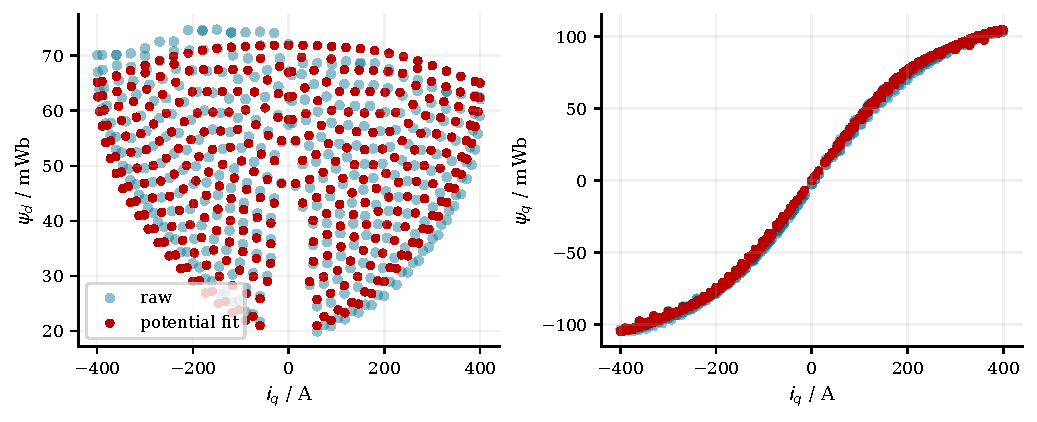
\includegraphics[width=\textwidth]{figures/real_reconstruction.pdf}
\caption{Raw and common-potential flux at each observed point, plotted against
q current. Points with different d current form distinct locations rather
than one fitted slice. Raw and reconstructed values are retained separately.}
\label{fig:real-reconstruction}\end{figure}
The full pointwise difference is exported as \texttt{real\_fit.csv}.
There is no extrapolation policy or experimental ground-truth correction claim.
